\chapter{系统设计与架构}
跨界服务将跨越不同行业、组织、价值链等边界的服务进行深度融合和模式创新,为用户提供多维度、高质量、富价值的跨界服务,成为现代服务业发
展的重要创新途径。跨界服务平台是各类跨界服务集成的支撑系统,相比传统的服务集成,跨界服务融合需开展模式、生态、环境、质量、价值等多维深度融合。
为将提出的算法与应用相结合,本文依托于国家重点研发计划专项《现代服务业共性关键技术研发及应用示范》的子课题《跨界服务集成方法与支撑载体》,
在跨界服务平台设计并实现了服务智能调用引擎,本章主要对跨界服务平台和智能调用引擎进行介绍。

\section{跨界服务系统}
本文作者所在的课题组系统性地研究了跨界服务相关理论,并形成了跨界服务原型系统JTangYdrail(图\ref{fig:jianmu}),
本节主要介绍系统整体架构以及跨界服务系统中两个核心模块服务交换机和服务路由器。
\begin{figure}[htbp]
    \centering
    
\includegraphics[width=6cm]{./images/jianmu.jpg}
    \caption{跨界服务系统 logo}
    \label{fig:jianmu}
  \end{figure}


  \begin{figure}[htbp]
    \centering
    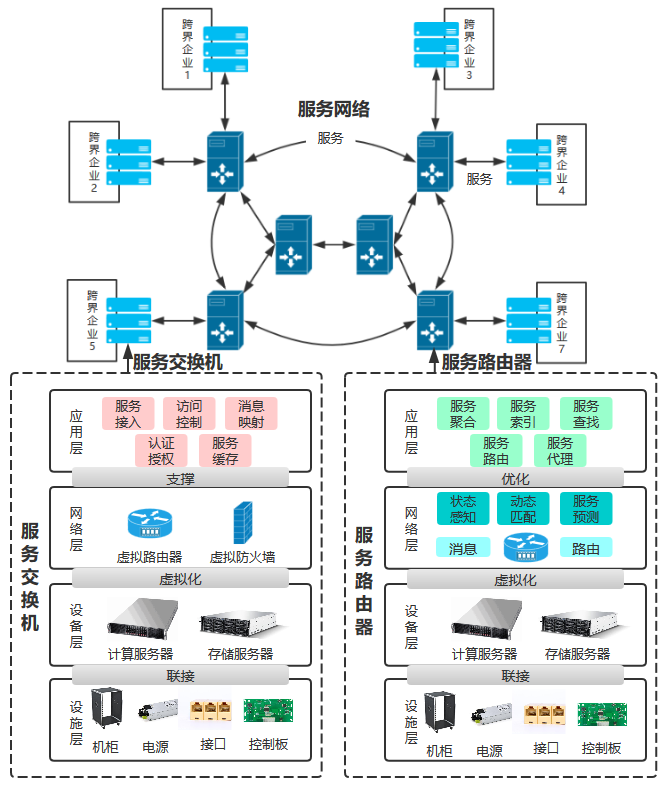
\includegraphics[width=10cm]{./images/system.png}
    \caption{JTangYdrail系统架构}
    \label{fig:jianmu}
  \end{figure}


  \begin{figure}[htbp]
    \centering
    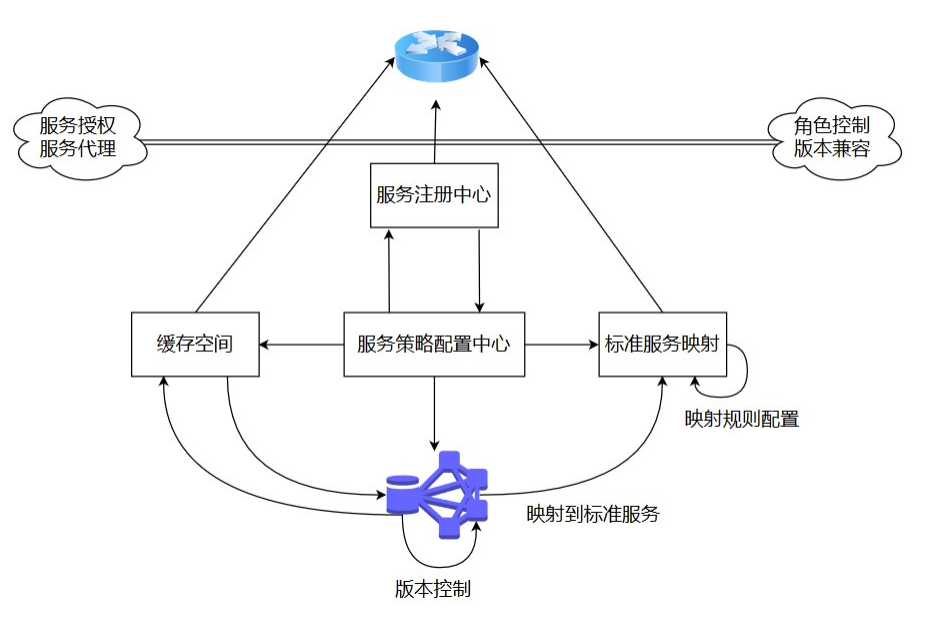
\includegraphics[width=10cm]{./images/switchboard.png}
    \caption{JTangYdrail 服务交换机软件架构}
    \label{fig:jianmu}
  \end{figure}

  \begin{figure}[htbp]
    \centering
    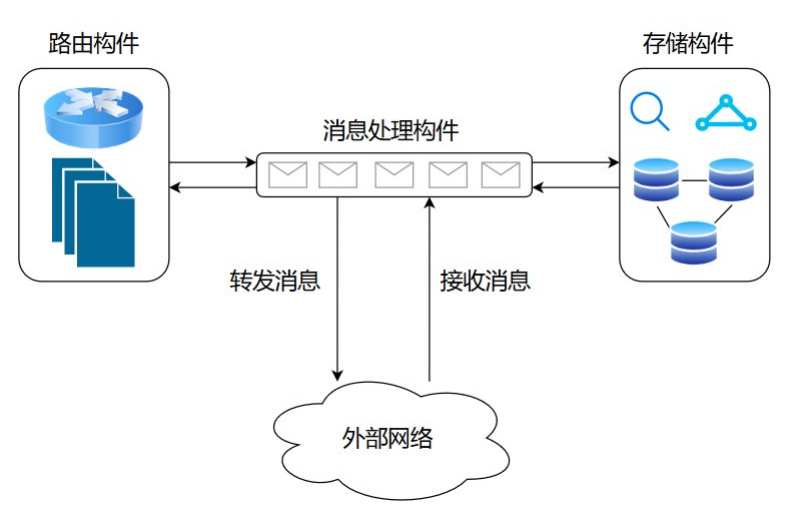
\includegraphics[width=10cm]{./images/router.png}
    \caption{JTangYdrail 服务路由器软件架构}
    \label{fig:jianmu}
  \end{figure}


  
  
  \section{服务智能调用引擎}

  \section{系统原型展示}
